

\subsection{Menu Description}
When the game is started, the user is presented with a menu. The layout for the menu is defined with a layout XML-file. Using XML is the most common way to control layout for Android applications.\cite{android:ui} This menu is represented programitically with the MenuActivity class, which extends the Activity class. An activity in Android is in most cases "what you see", and defines where the user is in the application. A user can navigate between activities through the use an Activity stack, which defines the most recent activities, thus allowing to navigate backwards. This is generally done with the "back" button on the phone, or customized buttons/events introduced by the developer of the application.\cite{android:activity}

The menu activity consists of a "Play" button, which starts the game. When this button is pressed, a new activity is started -- PlayActivity. This activity starts the game. When the player has died, or has pressed the back button, PlayActivity is paused, and MenuActivity is resumed. This can be further explained with the Activity lifecycle in figure ~\ref{fig:activityLifecycle}, which is provided by the Android Developer Guide.


\begin{figure} [h]
	\center
		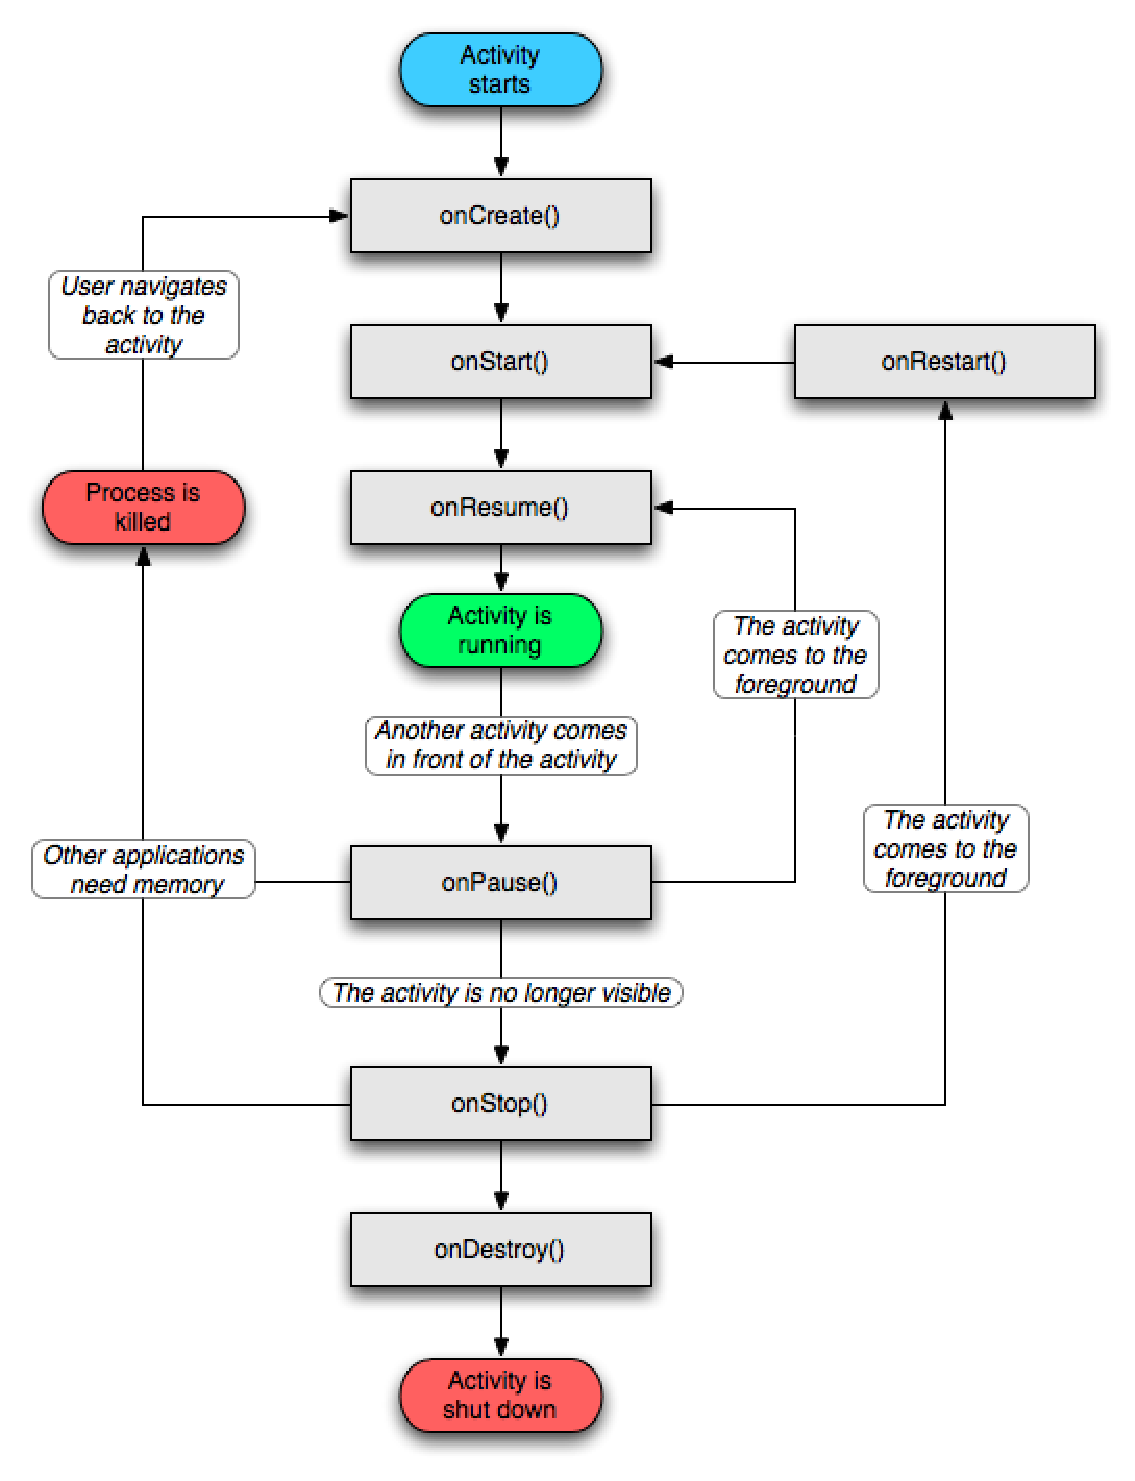
\includegraphics[scale=0.5]{main/figures/activity_lifecycle}
		\caption{Activity Lifecycle\cite{android:activity}}
		\label{fig:activityLifecycle}
\end{figure}

\subsection{Game Description}
When PlayActivity is started from the menu, the game starts. Upon creating the activity, onCreate is called and initializes our game object, as explained in figure \ref{fig:activityLifecycle}. The game object consists of a state, which again consists of different layers. Figure \ref{fig:structure} displays an overview over the most important components of the game. 

The view of the game is displayed using the Sheep framework, through the use of a canvas, which decide what is shown on the display. The game object calls the update and draw methods frequently, thus allowing animation and movement. The update and draw methods are called in a chain downwards in the hierarchy of classes, which are further explained in the architectural report.\cite{arcReport}

\subsection{Touch Gestures}
The GestureController class listens for touch gesture made by the user. The gestures detected are pinch zoom (two fingers moving away or towards each other) and long press. When initiating a pinch zoom, the canvas is enlarged through the scale method. When a long press is detected, a dialogbox to create tower will appear. The dialog layout is defined in a XML layout file. After clicking on a tower, the tower will be placed at the position which the long press appeared.

The user will not be able to zoom in more than 3 times normal zoom level, and out more than the size of the map, which is the starting zoom level for any screen. The zoom level is calculated with the formula in equation \ref{eq_zoom}. If the user tries to zoom outside these values, the zoom level will be set to the respective max or min level.


\begin{equation}\label{eq_zoom}
	\frac{displaysize}{mapsize} < zoom level < 3
\end{equation}

\subsection{Music}
Music is played through the use of the MediaPlayer class, which is initiated when PlayActivity is started/resumed, and paused when the game is no longer in focus.

\subsection{Tiled Map}
A lot of the modifiability requirements are concerned about game content. One should be able to change, add or delete content with ease. In the context of the game map, this means that a map editor should be availible for the map designers. Hard-coding a map directly into the programming language is out of the question. Furthermore, the map should be stored in a flexible data format which is easy processs programatically. 

These goals are achieved by basing the map functionality on the Tiled Map Editor.\cite{mapeditor} It is an open source, general purpose map editor, which handles maps stored in the XML data format\footnote{The file extension is *.tmx}. It is written in C++ using the Qt application framework, but it is also ported to Java\footnote{The Java version is no longer maintained officially}, which is what we used. Unfortunately, the code had a lot of dependencies on the Swing API, and this is not a part of the Android API. In other words, the functionality had to be ported to Android. Only a subset of the functionality was ported to the application; about 60\% of the original code. This means that the map has to be designed on a desktop computer running a standard Java Virtual Machine (JVM), and the produced *.tmx file can then be read (parsed) on the Android Dalvik Virtual Machine (supporting the Android API).

\subsubsection{Creating And Parsing Map}\label{parsingmap}
A game map is 2-dimensional and composed of small square images called tiles. The map itself is referred to as a tiled map. In order to create a map, one first needs a tile set. This is basically a single image file which is constructed as a regular grid of smaller images. This image is then cut along the grid lines into separate images. All of these new images constitutes the palette from which one can draw the map. This functionality resides in the Tiled Map Editor. In addition to drawing tiles, one can draw objects. These are typically not rendered, but only used as logical elements. This was used to define spawn, goal and waypoint areas in the map. With this, the map design process has become rather effortless and the dataformat is very flexible. The map creation process was considered as satisfactory.

Representing arbitrary data structures with XML is easy, interpreting and parsing them is another story. The *.tmx files are structured as a tree. The DOM (Document Object Model) parser library was used to parse the map files. \cite{dom}


\subsection{Enemies}

The enemies in the game consists of streams of sprites moving from the spawn-area of the map in a set path to the goal-area of the map. There are four types of enemies, illustrated in figure \ref{fig:enemies}

\begin{figure}[htbp]
	\centering
		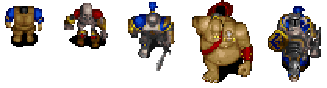
\includegraphics{main/figures/enemies}
	\caption{Enemies}
	\label{fig:enemies}
\end{figure}


An enemy is represented as an EnemySprite-object, which extends the class Sprite from the Sheep-framework. The Sprite-class contains functionality for drawing and updating a sprite on the screen. It also contains functions for setting an image as the visual representation, as well as functions for moving the sprite around the screen. 

In addition to the functionality already implemented in the Sprite-class, the EnemySprite contains properties such as hit-points, its status (when the hitpoints are dropped below zero, the sprite is considered dead), as well as information regarding the sprite's position on the map. It also has a visiblity-property, deciding whether the sprite should be visible on the screen. 

\subsubsection{Pathing}
As mentioned in section \ref{parsingmap}, the game maps contain information about spawn, goal and waypoint areas. Even information about which areas are walkable is coded into the map. This information is handled by the TowerDefenseMapLayer class. To construct a path, the elements are first ordered like this: $spawn, waypoint_1, waypoint_2, ..., waypoint_n, goal$. Then it is iterated over in this order, building a path between every two consecutive elements, and linking these paths together. The algorithm used is the A* search algorithm \cite{aima}, and the admissible heurestic is the manhattan distance \cite{wiki:manhattan}.

\subsection{Towers}
The towers are sprites of the type TowerSprite-object, and they extend the Sprite-class, just like the enemies. The difference between the towers and the enemies is that the towers does not move after they are spawned. Instead, the towers have an attack-animation which is performed in the same way as the animation for the enemies. The player can create four different towers in the game, which are illustrated in figure \ref{fig:towers}. 

\begin{figure}[htbp]
	\centering
		
\includegraphics{main/figures/towers}
	\caption{Towers}
	\label{fig:towers}
\end{figure}


All towers have different range, damage and price, which are defined in a class called "Globals". By having a Globals class with all the properties of each tower one can easily change the difficulty of the game, in order to achieve balance in the gameplay.


The towers frequently check for enemies in near proximity, and shoots if possible. The shooting functionality is further explained in detail by the following pseudocode.\newline


\begin{algorithmic}
\FORALL{Towers}
	\IF{Tower.isFiring}
		\IF{Tower.getTarget.isDead}
			\item Stop firing
		\ELSIF{\NOT targetInRange}
			\item Stop firing
		\ELSE
			\item Keep firing at target
		\ENDIF
	\ELSE
		\FORALL{enemies}
			\IF{targetInRange(tower, enemy) and \NOT enemy.isDead}
				\item Fire at enemy
				\item Stop looping through enemies
			\ENDIF
		\ENDFOR
	\ENDIF
\ENDFOR
\end{algorithmic}

Here the list of towers is iterated through, checking if it should change target or not. When checking for a new target, the list of enemies is iterated through. The first enemy of the list is chosen, then the for loop is stopped. Since the first enemy in the list is chosen, the enemy closest to the goal is chosen. The targetInRange function is calculated with the formula explained in equation \ref{eq:targetInRange}. When iterating through the tower and enemy lists, synchronized is called on both lists, to lock the access to these lists to the current thread. This is further explained in section \ref{threading}.

\begin{equation}\label{eq:targetInRange}
	(TowerX - enemyX)^2 +(TowerY - EnemyY)^2 <= tower range^2
\end{equation}

Here X and Y refers to the coordinates of the towers and enemies, while tower range refers to the range of the different towers.

\begin{figure}[htbp]
	\centering
		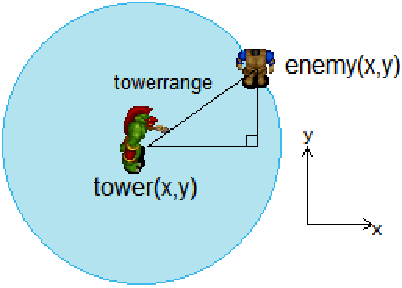
\includegraphics{main/figures/range}
		\caption{Attack range of an axe thrower}
	\label{fig:range}
\end{figure}

Figure \ref{fig:range} shows an example of the attack range of the axe thrower tower.


\subsubsection{Animation}

By adding several images, the sprite can be animated. In our case the sprite has images which makes the sprite seem as it is walking and attacking, as illustrated in figure \ref{fig:axeanimation}. Animation is accomplished by switching the image giving the visual representation of the sprite in a set frequency. 

\begin{figure}[htbp]
	\centering
		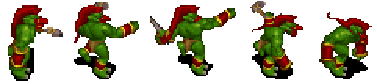
\includegraphics{main/figures/axeanimation}
		\caption{Axe thrower attack animation}
	\label{fig:axeanimation}
\end{figure}


The images of a EnemySprite-object is collected in an EnemyImageStructure-instance. This is a structure containing all the images connected to a sprite, including five animation images and an image illustrating that the sprite is dead.

